\documentclass[11pt, a4paper]{article}
\usepackage[latin1]{inputenc}
\usepackage{pgfplots}
\usepackage{pgfplotstable}
\usepackage{float}
\pgfplotsset{width=0.85\textwidth ,compat=1.9}
\usepackage[dutch]{babel}
\usepackage{csquotes}
\usepackage{amsmath}
\usepackage[toc,page]{appendix}
\usepackage{amsfonts}
\usepackage{amssymb}
\usepackage{graphicx}
\usepackage{caption}
\usepackage[backend=biber, style=numeric, citestyle=numeric-comp, sorting = none]{biblatex}
\author{Stef Tweepenninckx, r0677232}
\title{Practicum 1: Sorteeralgoritmes}


%define printtitle
\makeatletter
\def\printtitle{                 
    {\large \@title}} 
\makeatother

%define printauthor
\makeatletter                       
\def\printauthor{                  
    {\large \@author}}              
\makeatother

\begin{document}
\begin{titlepage}
\newcommand{\HRule}{\rule{\linewidth}{0.5mm}} 
\center 
\textsc{\LARGE Gegevensstructuren en algoritmen}\\[1.5cm] 
\HRule \\[0.4cm]

{\huge \bfseries \printtitle}\\[0.4cm] 
\HRule \\[0.4cm]

\Large \emph{Author:}\\
 \textsc{\printauthor}\\[3cm]

{\large \textsc{1 mei 2018}}\\[3cm] 

\vfill 
\end{titlepage}

\section*{Inleiding}

\section*{Overzicht}
\begin{table}[ht]
\centering
\label{my-label}
\begin{tabular}{|cccc|}
\hline
Puzzel       & Aantal vergelijkingen & Hamming (s)        & Manhattan (s) \\ \hline
puzzle28.txt & 28                    & 2.435              & 0.113         \\
puzzle30.txt & 30                    & 3.920              & 0.140         \\
puzzle32.txt & 32                    & \textgreater 5 min & 4.803         \\
puzzle34.txt & 34                    & \textgreater 5 min & 1.093         \\
puzzle36.txt & 36                    & \textgreater 5 min & 14.168        \\
puzzle38.txt & 38                    & \textgreater 5 min & 10.885        \\
puzzle40.txt & 40                    & \textgreater 5 min & 2.490         \\
puzzle42.txt & 42                    & \textgreater 5 min & 8.528         \\ \hline
\end{tabular}
\captionsetup{justification=centering,margin=2cm}
\caption{Resultaten experiment met Hamming en Manhattan prioriteitsfunctie}
\end{table}
\section*{Tijdscomplexiteit Hamming}
De Hamming prioriteitsfunctie kijkt naar het aantal elementen die op de foute plaats staat. We lopen over de hele puzzel en vergelijken de waarde op een bepaalde positie i,j met de verwachte waarde. Als deze 2 waarden niet overeenkomen verhogen we het resultaat.\\
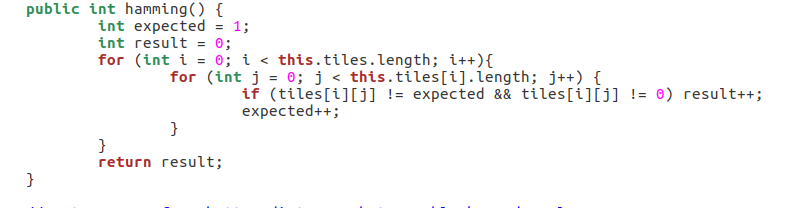
\includegraphics[width=\textwidth]{hamming}\\
In mijn implementatie van de Hamming functie gebruik ik twee for-lussen die beide van 0 tot N lopen. Bij elke iteratie zijn er maximaal twee array accesses nodig. In dit worst-case geval is de tijdscomplexiteit $\sim 2\cdot N^2$.\\
In het beste geval (de puzzel is al opgelost) wordt de 2\textsuperscript{e} array access slechts 1 keer uitgevoerd, bij het 0 vakje (dit kan nooit gelijk zijn aan de variabele \emph{expected}). Bij de gewone vakjes is de if-clausule al gefalsifi\"eerd door de 1\textsuperscript{e} array access en wordt de 2\textsuperscript{e} dus niet uitgevoerd. De best-case tijdscomplexiteit is dus $\sim N^2 + 1$.
\section*{Tijdscomplexiteit Manhattan}
\section*{isSolvable}
\section*{Borden in geheugen}
\section*{Worst-case tijdscomplexiteit}
\section*{Betere prioriteitsfuncties}
\section*{Tijd, geheugen of algoritme?}
\section*{Effici\"ent algoritme}


\end{document}
